\chapter{Impact Analysis}
In questa sezione si presenterà una previsione dell'impatto che la modifica richiesta avrà sugli artefatti del sistema esistente. In particolar modo si cercherà di individuare le classi (codice sorgente) che dovranno essere modificate per integrare le funzionalità richieste.

\paragraph{}
Dato che si è scelto di implementare un sistema ex novo le cui funzionalità andranno ad affiancare e integrare quelle del sistema esistente, a livello di codice sorgente l'impatto sarà pari a zero.

RepominerEvo andrà ad interagire con esso solamente al layer di gestione dei dati, in quanto andrà a utilizzare le informazioni estrapolate e memorizzate da Repominer per implementare nuove funzionalità. Si può ragionevolmente dedurre quindi che l'impatto sul sistema esistente andrà gestito unicamente a livello di database.

Dato che dovranno essere implementate nuove metriche di natura più complessa ed articolata, si presume che sarà necessaria la modifica di alcune tabelle e di alcuni campi nel database esistente.
\\

Nella figura \ref{fig:sie} di pagina \pageref{fig:sie} riportiamo la relazioni e le tabelle più significative al momento corrente ai fini delle metriche da implementare.
\\
In particolare, ipotizziamo che lo Starting Impact Set conterrà la tabella:
\begin{itemize}
\item \textit{`metrics`}
\end{itemize}
Si è pensato, dovendo estendere le metriche già calcolate in Repominer con nuove metriche, distinte in metriche di pacchetto e metriche di progetto, di dover prevedere la creazione di due nuove tabelle: 
\begin{itemize}
\item \textit{`package\_metrics`}
\item \textit{`project\_metrics`}
\end{itemize}

Nella figura \ref{fig:dettaglio} di pagina \pageref{fig:dettaglio} mostriamo le nuove relazioni ipotizzate che si verranno a creare. Si precisa che tali nuove relazioni non avranno alcuna influenza con la struttura del database preesistente.

\begin{figure}[t]
	\centering
	%width=.5\textwidth
	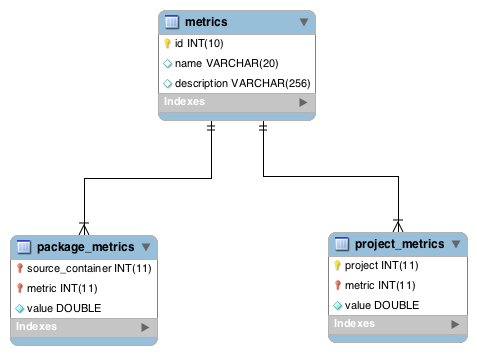
\includegraphics[width=.5\textwidth]{img/dettaglio.png}
	\caption{Dettaglio delle relazioni da instaurare}\label{fig:dettaglio}
\end{figure}

\begin{figure}[b]
	\centering
	%width=.5\textwidth
	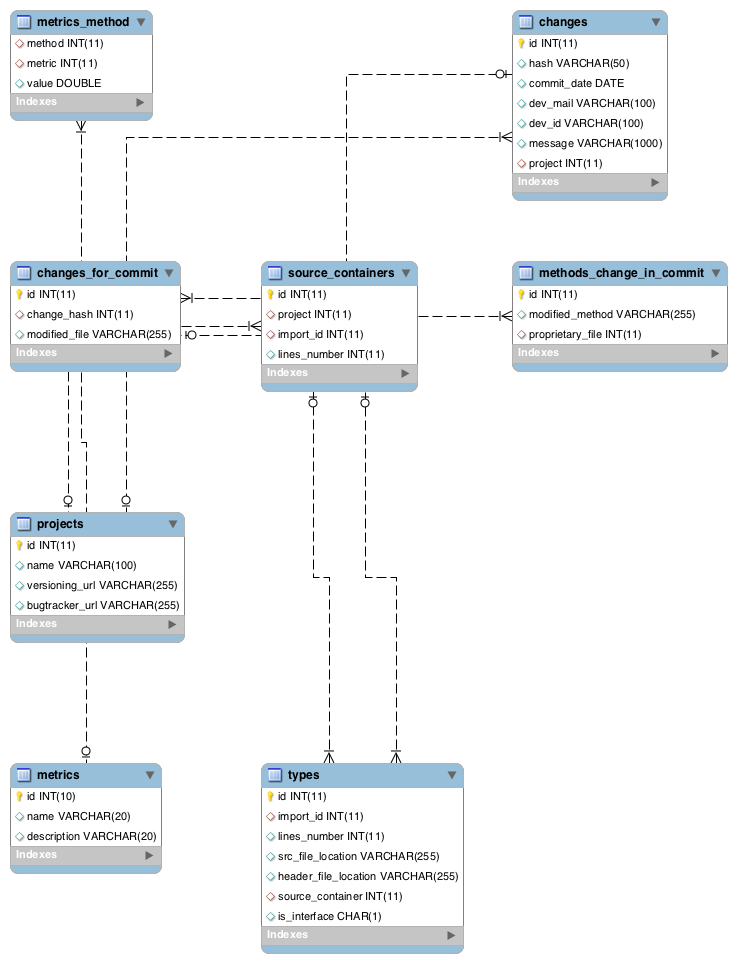
\includegraphics[width=\textwidth]{img/sieImportant.png}
	\caption{Schema relazionale del DB con le relazioni princpalmente interessate dall'analisi}\label{fig:sie}
\end{figure}

A seguito di un'analisi approfondita, è stato individuato il Candidate Impact Set nell'unica tabella: 
\begin{itemize}
\item \textit{`metrics`}
\end{itemize}
A seguito di tale analisi rimangono valide le considerazioni sopra esposte riguardo le nuove tabelle da creare e le relazioni da instaurare con \textit{`metrics`}.
\\

Una valutazione dettagliata dei risultati di questa analisi sarà presentata in un report separato dopo l'implementazione completa delle modifiche.